\section{Evaluation of Approximation Variance}
\label{sec:estimation-variance}

In this section we will derive a rough quantitaitve estimate of variance of $ \hat f_i$
and then support its credibility by experimental results.

\subsection{Derivation of $Var(\hat f_i)$}
Using the observation that values $w_i^*$ chosen by Kmerlight often correspond
to the analytical $w^+$ and the observation that the value of analytical $w^+$ is a constant
for all $i=1, 2, \dots, m$, we will approximate Kmerlight's variance by a variance
of $t_i^{(w^+)}$. This variance approximation will be even more accurate for our modified
Kmerlight. 

In this section we will denote
$w^+$ simply as $w$, since we will not use any specific property of $w^+$.

The number of collision-free $k$-mers is equal to the number of collision-free counters
as each collision-free counter stores a single $k$-mer. Thus we will use the symbol
$t_i^{(w)}$ to denote both quantities and  from (\ref{eq:ti}) it holds that 
$E(t_i^{(w)}) = f_i/2^w \cdot (1 - 1/r)^{F_0/2^w-1}$.

\paragraph{Sampling View}
In order to approximate the variance of estimator $\hat f_i$ we will consider
$t_i^{(w)}$ to follow a binomial distribution $Bin(f_i, p_s)$, where
$p_s = 1/2^w \cdot (1 - 1/r)^{F_0/2^w-1}$.
This simplification corresponds to a simple sampling process in which we sample each of $f_i$ 
$k$-mers with probability $p_s$ (sampling probability) and we discard each $k$-mer
with probability $1 - p_s$. Note that this approach ignores the fact that the events
of $k$-mers remaining collision-free are not independent. 

Since a random variable following $Bin(n, p)$ has variance of $np(1-p)$, 
$Var(t_i^{(w)}) = f_i \cdot p_s \cdot (1-p_s)$. The estimate of $f_i$ is obtained
as $t_i / p_s$, so

\begin{equation} \label{eq:varhatfi}
Var(\hat f_i) = Var \left( \frac{t_i}{p_s} \right) = \frac{1}{p_s^2}
\cdot Var(t_i) = \frac{f_i \cdot (1 - p_s)}{p_s}
\end{equation}

\paragraph{Effect of Medians}
Kmerlight chooses the estimate $\hat f_i$ as a median of estimates of $t$ 
independent sketches: $\hat f_i = \mathrm{med}(\hat f_i^{(1)}, \dots \hat f_i^{(t)})$.

To incorporate the effect of medians, we will use the claim that for a continuous random
variable with a density function $f(x)$ and mean $\bar x$ its sample median from a sample of
size $n$ is asymptotically\footnote{Rider \cite{Rider1960} have shown that 
even for a sample of only $7$ observations, the relative error of this approximation is only
circa 6\% for a normal random variable.} normal \cite{WikiMedian}:

\begin{equation} \label{eq:median}
\mathrm{med}(x) ~\dot\sim~ N\left(\bar x, \frac{1}{4nf(\bar x)^2}\right)
\end{equation}

As the binomial distribution of $t_i^{(w)}$ is a discrete distribution and does
not have a density function, we will approximate $Bin(f_i, p_s)$ with
$N(\mu = f_i p_s, \sigma^2 = f_i p_s(1-p_s))$. The density function of normal distribution
in its mean $\mu$ is $\frac{1}{\sqrt{2\pi\sigma^2}} e^{-\frac{(\mu - \mu)^2}{2\sigma^2}}$
which is $\frac{1}{\sqrt{2\pi\sigma^2}}$.

Using the two previous approximations (\ref{eq:varhatfi}), (\ref{eq:median}), 
variance of $\hat f_i$ selected as a median of $t$ instances can be derived as follows:

\begin{equation} \label{eq:variance}
Var(\hat f_i) \approx \left( 4t\frac{1}{2\pi Var(\hat f_i^{(l)})}) \right)^{-1} =
\frac{2\pi}{4t} Var(\hat f_i^{(l)}) = \frac{\pi}{2t} \frac{f_i \cdot (1 - p_s)}{p_s}
\end{equation}


\subsection{Comparison With Experiments}
In order to validate our estimate of variance we compare our theoretical model of the distribution 
of $\hat f_i$ with the experimentally obtained distribution.

We ran our modified Kmerlight with $t=7$ instances in 300 trials on the data presented in 
section \ref{sec:error-characteristics}. In Figure \ref{img:estimated-pdf}
we present histograms of values of $\hat f_i$ for multiple values of $f_i$\footnote{
The values $i = 6,10,13,16,32,23,2,1$ were selected as follows. We sorted the values 
$f_i$ in increasing order and then we selected each eighth value. Since the values of
$f_1, f_2$ differ from other $f_i$ by orders of magnitude, we decided to also include $i=1,2$.}.
In Figure \ref{img:estimated-cdf} we present empirical cumulative distribution functions
of the same data. 

We compare these histograms with two normal distributions. The best normal fit is a gaussian
with its mean and standard deviation obtained directly from the observed values of $\hat f_i$.
The plotted theoretical prediction uses the exact value of $f_i$ as its mean $\mu$ and
the variance $\sigma^2$ is calculated according to (\ref{eq:variance}) with use of exact values of 
$f_i$ and $F_0$. 

\medskip

Our theory does not model the mean value of Kmerlight's estimates. We assume that the estimates
$\hat f_i$ are unbiased and therefore we simply use $\mu = f_i$ and we focus on modified
Kmerlight. If we used one of the observed estimates $\hat f_i$ as the parameter $\mu$, the
fluctuation of $\hat f_i$ would shift the plotted theoretivcal curves to the side and thus it 
would make the comparison less clear. 

In practice, estimates of $f_i$ and $F_0$ will be used to calculate the variance. We also might
have used estimates $\hat f_i, \hat F_0$ from a single trial to calculate the variance estimate, 
but by using the average $\hat f_i$ we investigate the average estimate of variance.   

We also used the original Kmerlight to produce the values $\hat f_i$ in another experiment.
Since we do not model the bias of Kmerlight's estimates, to make the histogram comparable
to our theory, we had to use the sample mean of $\hat f_i$ as the parameter $\mu$.
With this adjustment we were able to observe the same phenomena as those presented in figures and 
described below.


\begin{figure}[h]
\centerline{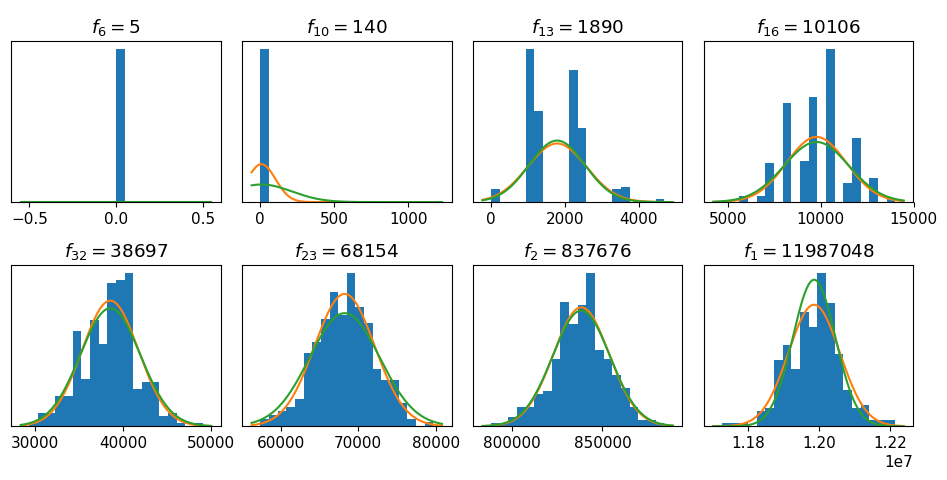
\includegraphics[width=1\textwidth, trim={0cm, 0.1cm, 0cm, 0cm}, clip]{images/pdf2.png}}
\caption[Density functions of $\hat f_i$]{Empirical probability densities (blue histograms), best
normal fits (orange lines) and theoretical estimates (green) of distributions of $\hat f_i$
for multiple abundances. Histograms come from 300 runs of modified Kmerlight.
Horizontal axes display the values of estimates $\hat f_i$.}
\label{img:estimated-pdf}
\end{figure}

\begin{figure}[h!]
\centerline{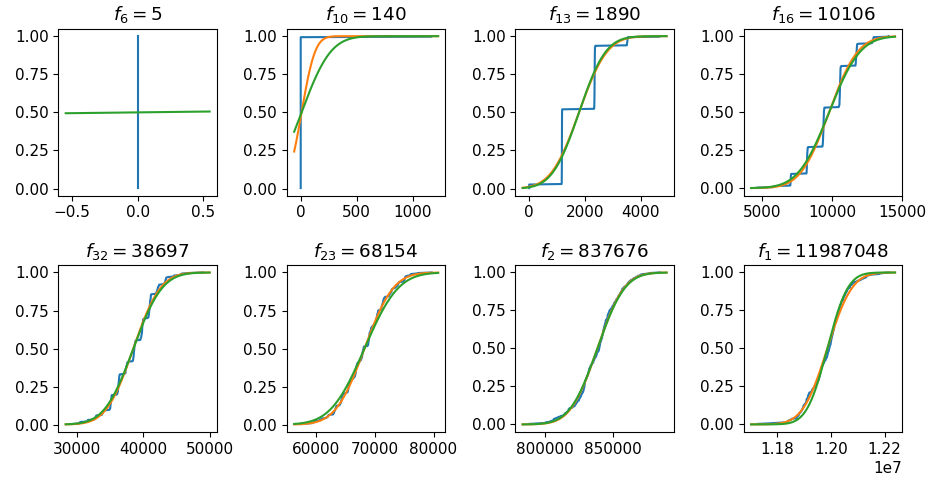
\includegraphics[width=1\textwidth, trim={0cm, 0.1cm, 0cm, 0cm}, clip]{images/cdf2.png}}
\caption[Distribution functions of $\hat f_i$]{Empirical cumulative distribution functions (blue), 
best normal fits (orange), theoretical estimates (green).}
\label{img:estimated-cdf}
\end{figure}

Note first that for this dataset, $w^+ = 9$ and thus the sampling probabilty $p_s$
(introduced in the previous section \ref{sec:estimation-variance}) is approximately
$1/2^9 \cdot \frac{1}{2} \approx 1/1000 $ when we use the upper bound from (\ref{eq:wplusbounds}).

\paragraph{The lowest $f_i$ values, $E(t_i) = f_i \cdot p_s < 1$}
For the lowest values of $f_i$ (e.g. $f_6, f_{10}$), 
no $k$-mers survive the collisions at level $w^+$ and thus $t_i = 0$ and $\hat f_i = 0$. 
As $f_{10}=140$ is only approximately ten times lower than $p_s$, we might expect at least
one $k$-mer to survive collisions in some of 300 trials. But since the final estimate is selected
as a median of seven instances, at least one $k$-mer must survive in at least four instances
in order to produce $t_i = 1$. Thus $\hat f_i = 0$. 

Since the estimates $\hat f_i$ are always zero, our estimates of variances for these $f_i$ are 
very unprecise.

\paragraph{Low $f_i$ values, $E(t_i) = f_i \cdot p_s \approx 1$}
For low values of $f_i$ (e.g. $f_{13}, f_{16}$), a very small number of $k$-mers hash
into collision-free counters at level $w_i^*$ or $w^+$. Therefore the
estimator $\hat f_i$ can reach only a limited set of discrete 
values (0 if no $k$-mer survives collisions, $1/p_s \approx 1000$ if one $k$-mer is in
collision-free counter, $2/p_s \approx 2000$ if two $k$-mers survive, \dots), as it can
be seen in Figure \ref{img:estimated-pdf}.

The approximation with normal distribution is not precise for these values $f_i$, since
the distribution of $\hat f_i$ is clearly discrete, but Figure \ref{img:estimated-cdf} shows
that our approximation can be used to estimate distribution functions (and thus approximate
$p$-values).

\paragraph{High $f_i$ values, $E(t_i) = f_i \cdot p_s \gg 1$}
For higher $f_i$, the estimator $\hat f_i$ reaches various values and the approximation with
normal distribution seems reasonable, as it can be seen from bottom rows of figures 
\ref{img:estimated-pdf} and \ref{img:estimated-cdf}.

\medskip

We also tried to apply Kolmogorov-Smirnov tests to test the normality of $\hat f_i$. Discrete
values of $\hat f_i$ create steps in cumulative distribution functions and therefore these
tests reject normality hypotheses for columns with fewer $k$-mers. KS tests reject normality
for $f_i < 20\,000$ with dataset of 300 trials and significance level of $5\%$. 

\medskip

From previous observations we conclude that the distribution of $\hat f_i$ can be approximated
by gaussian with variance calculated by (\ref{eq:variance}), althouh we are also aware of the
limitations of this approximation.

Finally we present the comparison of Kmerlight's variance and its theoretical prediction in
Figure \ref{img:std-theory}. Despite that our theoretical approximation is based on the 
analytical value of level $w^+$, it can also be used to predict the variance of the original 
Kmerlight algorithm. 

From the experiment we know that we can estimate standard deviation of Kmerlight's estimates
with accuracy higher than 5\% even for lower for values of $f_i,
(E(t_i) = f_i \cdot p_s \geq 1)$. The experiment further proves that an accurate estimate of
variance for the lowest values of $f_i < 100$ would be zero. 

\begin{figure}[h]
\centerline{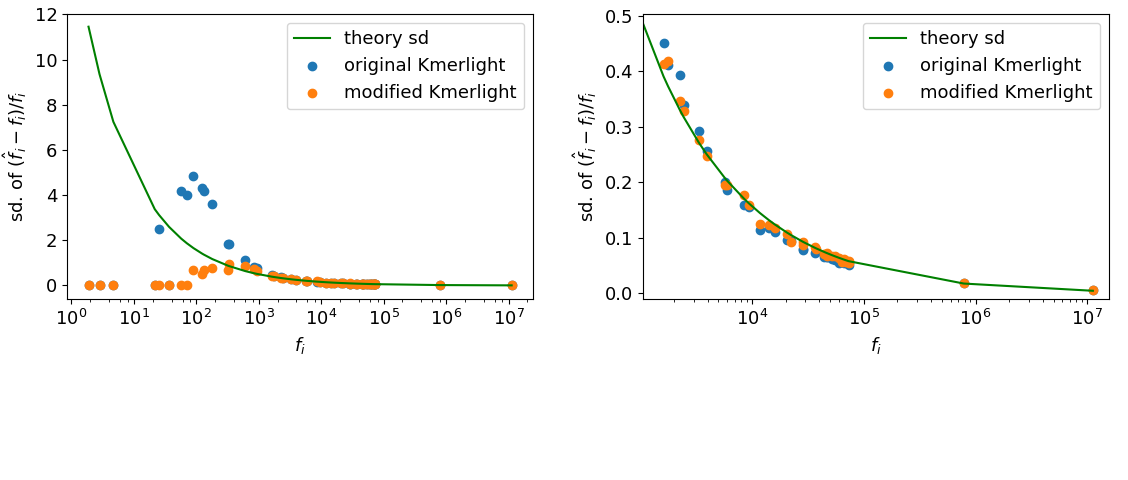
\includegraphics[width=1\textwidth, trim={0cm, 3.8cm, 0cm, 0cm}, clip]{images/std_deviations_comparison_theory2.png}}
\caption[Experimental and theoretical variance of Kmerlight]{The blue and orange points show 
standard deviations of relative errors $(\hat f_i - f_i) / f_i$ of estimates $\hat f_i$
computed by original and modified Kmerlight respectively in 300 runs on dataset from 
\ref{sec:error-characteristics}. The green line represents the approximation of standard
deviation calculated using (\ref{eq:variance}). The figure on the right is only a zoom of the figure
on the left.}
\label{img:std-theory}
\end{figure}

There is one more interesting thing that can be noticed in Figure \ref{img:std-theory},
the difference of variances for $f_i \in (100, 1000)$ between original and modified Kmerlight's
estimates. The original Kmerlight searches for a level $w$ that maximizes $t_i^{(w)}$ so
even if only one $k$-mer with abundance $i$ survives the collisions at any level of the sketch, 
Kmerlight will use it for estimation of $\hat f_i$. We did not include this effect into the
variance estimation, hence the estimates for these $f_i$ are not precise for the original Kmerlight.
